\documentclass{tk3-team}
\usepackage[caption=false,font=footnotesize]{subfig}


\begin{document}

\Ex{iLift}{\today}{Group G}%
                {Elmi Ali}{Satia Herfert}%
                {Omar Erminy}{Floriment Klinaku}%
                {Yiqun Chen}%

\section{Problem statement}

When going to the gym, one often faces problems that are hard to solve without ubiquitous technology. In order to make progress, it is essential to keep track of
\begin{itemize}
	\item what equipment you used,
	\item how much weight you used,
	\item what exercises you did,
	\item how many repetitions you did, and
	\item how well you performed the exercise.
\end{itemize}

The conventional solution would be to use pen and paper to write down your sessions, or use your smartphone for the same purpose. Usually people are too lazy to write down information about each set in detail and just write down how many sets they did with what weight, at most.

More problems with this are that you have keep track manually which hinders the training flow, and that you have to look for the right information in a probably suboptimal representation (not a table) on your paper. Some graphs displaying different statistics would also be very helpful so you can see your progress in a fast and descriptive way.

In addition, when using a paper, you don't have access to your statistics anywhere outside of the gym. If you want to train somewhere else, like at home, in a different city, or outside, that can be a big obstacle.

In order to know how well you performed each exercise you need a lot of experience or advice from a professional. Sadly, few gyms provide personal trainers that assist your, or that service is very expensive. As a novice and without assistance people often perform the exercises in a bad way that can sometimes even hurt them. Event with some experience performance can degrade over the course of your whole training and it would be nice being notified when that happens, so you can concentrate again on performing the exercise correctly.

\section{Solution}

Our solution is a ubiquitous system that attempts to solve all the problems enumerated above. Precisely it keeps track of exercises performed with what equipment and what weight, counts the repetitions for each set, gives qualitative life feedback, and also saves quantitative feedback (how many percent of repetitions were performed correctly?).

The additional requirements we have for our solution is that is requires minimal user interaction and does not hinder the training flow. In order for our solution to work seamlessly, some actions need to taken in the gym. Firstly, each user needs a personal RFID tag. As users normally already have membership cards equipped with some kind of tag, this should be no obstacle. Secondly, all the equipment for free training (dumbbells, kettle-bells, etc.) also need to be augmented with an RFID tag.

\subsection{Application flow}
The broad flow of a training session with our technology is as follows. When the user arrives in the gym he is given the device that he attaches to his arm (.NET Gadgeteer in our prototype). He logs into the device by scanning his membership card with the RFID reader included in the device. A screenshot of this can be seed in figure \ref{fig_screen_welcome}. The user can log out again immediately, or in a later moment.

When going to perform an exercise, first the piece of equipment must be chosen by scanning the RFID tag attached to the equipment. The corresponding screenshot can be seed in figure \ref{fig_screen_select_equipment}. After that, the user is presented with possible exercises that can be done with the piece of equipment just chosen, like in figure \ref{fig_screen_select_exercise}. Note that different types of equipment have different exercises associated with them, event though there are overlaps. Of course, if the user changes his mind, he can also cancel and scan a different equipment. The user now choses an exercises by clicking the touchscreen of the device.

Subsequently, as shown in figure \ref{fig_screen_start_exercise}, the device will tell the user to go into starting position, which is different depending on the chosen exercise. Since the sensors are calibrated in this position, it is essential that the user adopts the correct starting position. After that the device will start counting the repetitions the user does, and acknowledges each with a short beep noise. The current repetition count can be seen on the screen, as you can see in figure \ref{fig_screen_execute_exercise}. In addition, if the exercise is not performed optimally, a different sound will be played and a note on how to improve is also displayed on the screen. Once the user is done with the current set, he clicks that option on the touchscreen.

After each training set, a short summary will be presented to the user, informing him of repetitions, weight, equipment, and performance. Performance is the percent of repetitions performed optimally. An example can be seen in figure \ref{fig_screen_summary}. In the same moment , all the information is uploaded to a server, so it can be accessed later. %TODO assure that this is actually correct (performance shown)

\begin{figure*}[!t]
\centering
\subfloat[Welcome screen]{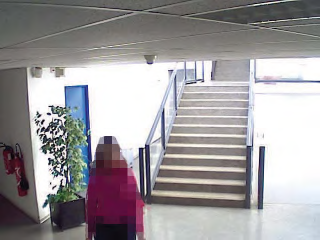
\includegraphics[width=2.0in]{img/sth}%
\label{fig_screen_welcome}}
\hfil
\subfloat[Select equipment screen]{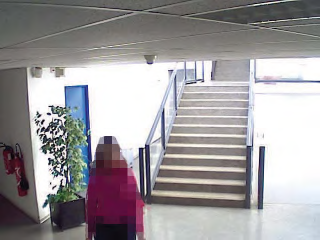
\includegraphics[width=2.0in]{img/sth}%
\label{fig_screen_select_equipment}}
\hfil
\subfloat[Select exercise screen]{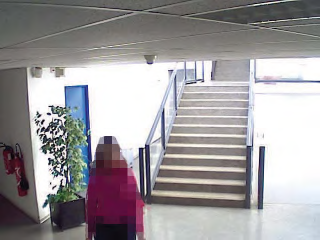
\includegraphics[width=2.0in]{img/sth}%
\label{fig_screen_select_exercise}}
\\
\subfloat[Start exercise screen]{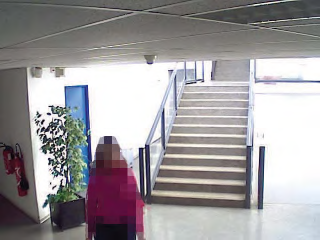
\includegraphics[width=2.0in]{img/sth}%
\label{fig_screen_start_exercise}}
\hfil
\subfloat[Execute exercise screen]{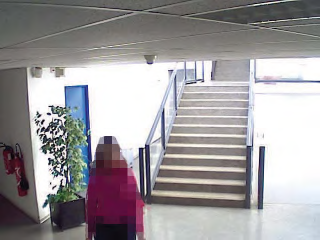
\includegraphics[width=2.0in]{img/sth}%
\label{fig_screen_execute_exercise}}
\hfil
\subfloat[Summany Screen]{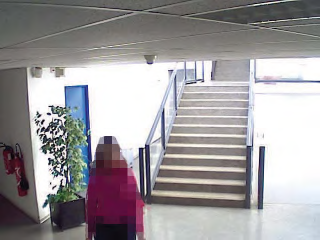
\includegraphics[width=2.0in]{img/sth}%
\label{fig_screen_summary}}
\caption{Screenshots from our application.}
\label{fig_screenshots}
\end{figure*}
%Welcome, SelectEquipment, SelectExercise, StartExercise, ExecuteExercise, Summary

Finally, the user can continue and perform more exercises and log out from the system when he is done with his training. At a later point, for example at home or during the next training session, the user can access all information of all previous trainings in an online interface with a computer or smartphone. In our prototype, a table summarizing all sets and some graphs are included. You can see the web interface in figure \ref{fig_web_screenshot}. %TODO assure that it are ``some'' graphs and not only one
%TODO include screenshot of website

\begin{figure*}[!t]
\centering
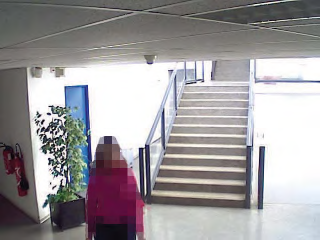
\includegraphics[width=\textwidth]{img/sth}
\caption{Screenshot from the web interface. %TODO explain
}
\label{fig_web_screenshot}
\end{figure*}

\section{Implementation}


\end{document}
